\documentclass[a4paper,10pt]{article}
\usepackage[a4paper, total={7in, 8in}]{geometry}
\setlength\parindent{0pt}
\usepackage[utf8]{inputenc}
\usepackage{graphicx}
\usepackage{caption}
\usepackage{subcaption}
\usepackage{amsmath}

\begin{document}

\begin{titlepage}
	\centering
	
\includegraphics[width=.6\textwidth]{liu-logo.png}\par
	\vfill
	{\scshape\Large TDDC17 ARTIFICIAL INTELLIGENCE\par}
	{\huge\bfseries Lab 4: Planning\par}
	\vspace{1cm}
	{\large\itshape Robin Andersson (roban591) \\ Lawrence Thanakumar Rajappa (lawra776)\par}
	\vfill
	{\large \today\par}
\end{titlepage}

\section*{Task 1}

We have chosen to model Shakey's domain.
In the domain we have the following six different objects:
\begin{itemize}
    \item \textbf{box}: a box that Shakey can push between connected rooms.
    \item \textbf{switch}: a light switch that can be turned on or off.
    \item \textbf{room}: a room where a light switch, object, box or Shakey can be.
    \item \textbf{shakey}: Shakey the robot.
    \item \textbf{object}: a small object that Shakey can hold.
    \item \textbf{gripper}: a gripper that Shakey can use to hold a small object.
\end{itemize}
The reason we chose these objects are because they are all required to model the domain since
we need boxes that can be moved, light switches that can be turned on and off, rooms where Shakey
and items can be placed, Shakey to track where it is, small objects so they can be moved and grippers
so Shakey can hold small objects.

We also have the following nine predicates:
\begin{itemize}
    \item \textbf{adjacent}: specifies wether two rooms are connected.
    \item \textbf{wide-entrance}: specifies wether the two rooms that are connected have a wide door.
    \item \textbf{box-at}: specifies if a specific box is in a specific room.
    \item \textbf{shakey-at}: specifies if Shakey is in a specific room.
    \item \textbf{switch-at}: specifies if a specific light switch is in a specific room.
    \item \textbf{object-at}: specifies if a specific small object is in a specific room.
    \item \textbf{light}: specifies wether a specific room is lit.
    \item \textbf{holding}: specifies if a specific gripper holds a specific small object.
    \item \textbf{empty}: specifies if a specific gripper is not holding anything.
\end{itemize}
These predicates were needed so we could specify which rooms that were connected and wether a box 
could be moved through these connected rooms. 
We also had to know where all items are located. 
Then the light was needed to determine wether small objects could be picked up. 
Finally, holding as well as empty were needed to allow Shakey to move the small objects around.
One predicate that could have been added is ''box\_under\_switch'', however, since the box already is
in the same room as the switch one could think of the box being moved under the light switch whenever
the light switch is going to be pressed.

Finally we have the following seven actions:
\begin{itemize}
    \item \textbf{move}: moves Shakey from one room to another if Shakey is in the first room and there is a door between the rooms.
    \item \textbf{lights-on}: Shakey turns on the lights in a room if there is a box and a light switch in the room.
    \item \textbf{turn-light-off}: Shakey turns the lights off in a room if there is a box and a light switch in the room.
    \item \textbf{move-box}: Shakey moves a box from one room to another if the rooms are connected with a wide door and the box is in the first room.
    \item \textbf{pick-up}: Shakey picks up a small object in one of its grippers if the light is on in the room and the object is in the same room as Shakey.
    \item \textbf{put-down}: Shakey puts down a small object from one of its grippers if the object is actually held in one of Shakey's grippers.
\end{itemize}
The move action was needed to allow Shakey to move between the different rooms. 
The actions related to light switches were needed to allow Shakey to turn on and off the lights in the rooms. 
Shakey also had to be able to move the boxes between the rooms in case there for instance only is one box and all rooms have to be lit. 
Finally, for Shakey to be able to pickup small objects an action for that was needed as well as an action for putting them down so new objects could be picked up.


\section*{Task 2}

\subsection*{Empirical Investigation}

\subsubsection*{1. Comparing heuristics, problem 03.}

\textbf{1.2}

From figure \ref{fig:p03-40} the Fast Forward heuristic has explored one path deeply since it selects the expanded and unvisited node with the lowest heuristic value in the queue. 
The Goal count heuristic has explored many paths shallowly since it chooses one of the expanded and unvisited nodes that has the lowest number of facts left to achieve.

\begin{figure}
    \centering
    \begin{subfigure}{.5\textwidth}
        \centering
        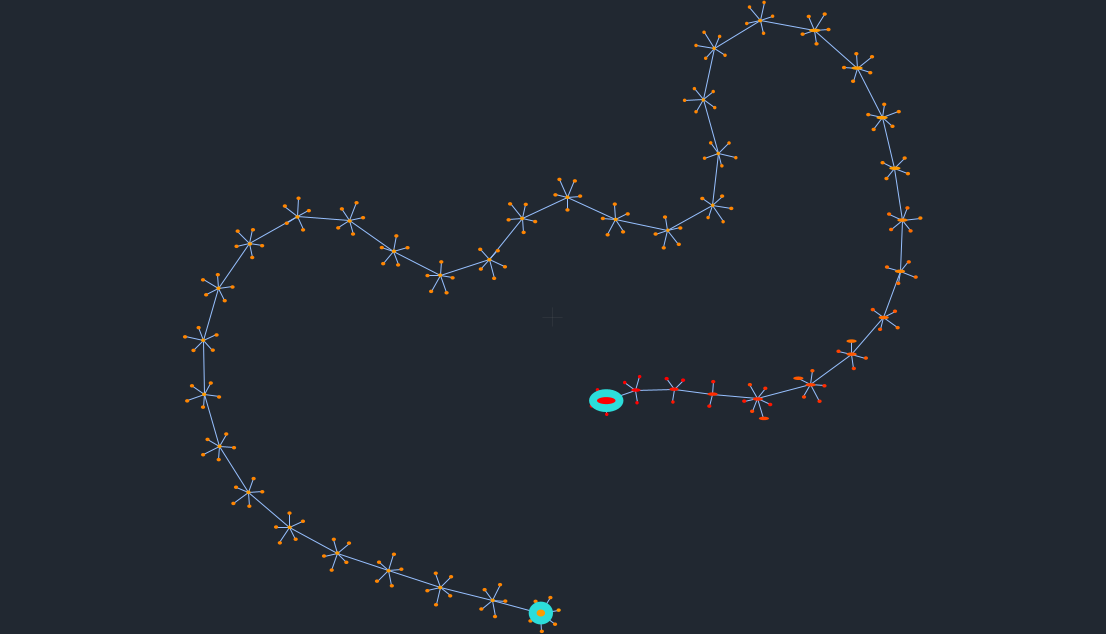
\includegraphics[width=.9\linewidth]{p03-ff-40.png}
        \caption{Fast forward heuristic.}
    \end{subfigure}%
    \begin{subfigure}{.5\textwidth}
        \centering
        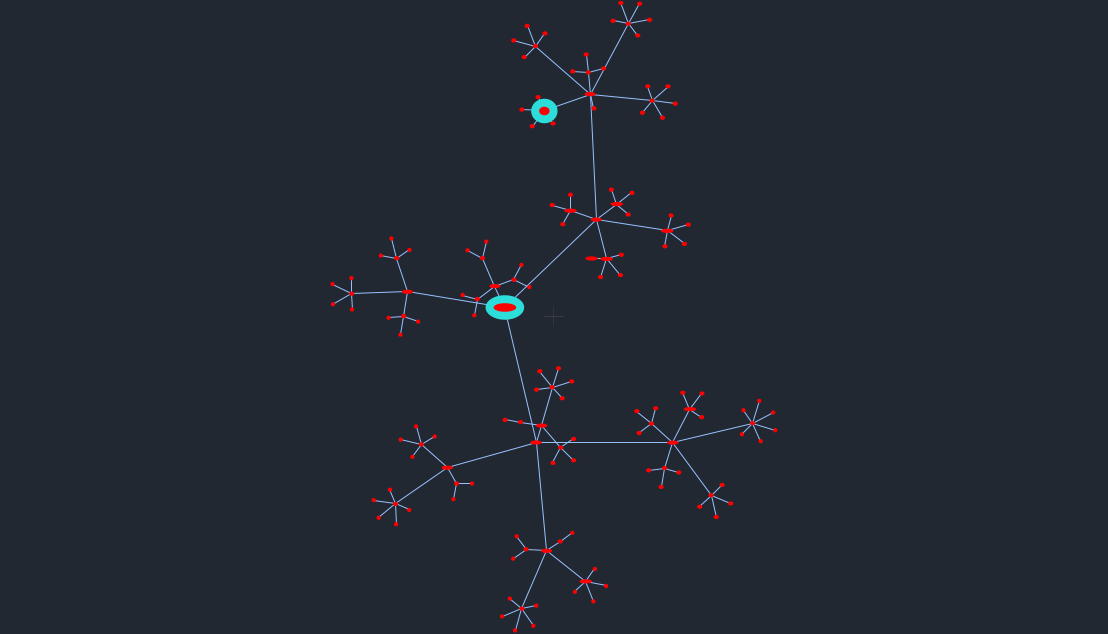
\includegraphics[width=.9\linewidth]{p03-gc-40.png}
        \caption{Goal count heuristic.}
    \end{subfigure}
    \caption{Problem 03 at step 40.} 
    \label{fig:p03-40}
\end{figure}

\textbf{1.3}

The Fast Forward heuristic has used all of the actions (load, unload and drive).
The Goal count heuristic has just used the actions load and drive.

\textbf{1.4}

The following nodes from 1.2 are used in the final plan: 0, 1, 8, 12, 13, 19, 26, 32 and 38.

\subsubsection*{2. Comparing heuristics, problem 02.}

\textbf{2.2}

The Fast Forward heuristic finds a new lower value for the main heuristic function in time step 7.
The Goal counter heuristic finds a new lower value for the main heuristic function in time step 3.

\textbf{2.3}

The Goal counter heuristic has six goal facts left to achieve.

\textbf{2.4}

The solution never increases the value of the goal count heuristic between states, it either statys 
the same or decreases.

\subsubsection*{3. Run one of the configurations on your own domain and problem.}

Running the fast forward heuristic on our first problem is quite similar to problem 02,
the only difference is that at time step 10 it decides to visit node 23 and then at time step 11 goes to node 24 which is connected to node 22 making node 23 unnecessary to reach the goal.
However it does make sense since it there tries to move Shakey to from room 3 to room 1, but since there are no boxes there it finds out that node 22 which is moving a box from room 3 to room 2 is much more effective.

\subsection*{Examination, Task 2}

\textbf{The statistics from using the different configurations to solve the given problems. Was any configuration better than the other? Was it better on everything or just on some problems?}

One configuration was not better than any other since it all depends on how the problems and 
domains are formulated. For instance, GC better than FF for problem 03, but FF was better than
GC for problem 02.

\textbf{Are your findings applicable to all the infinite many possible domains and problems? If so why? Else, why not? }

Yes the findings are applicable to all the infinite many possible domains and problems since it all boils down to how the problems and domains are setup. Some problems and domains may be well made for
specific configurations while being horrible for other configurations.

\end{document}